\begin{section}{General}
	Here we will specify important elements that are used across the application.
	\begin{subsection}{Default Management Table Form}
		This is specific page that is available to the organizer, but is an important
		element that is used in most of these pages.
		\begin{figure}[h]
		  \centering
			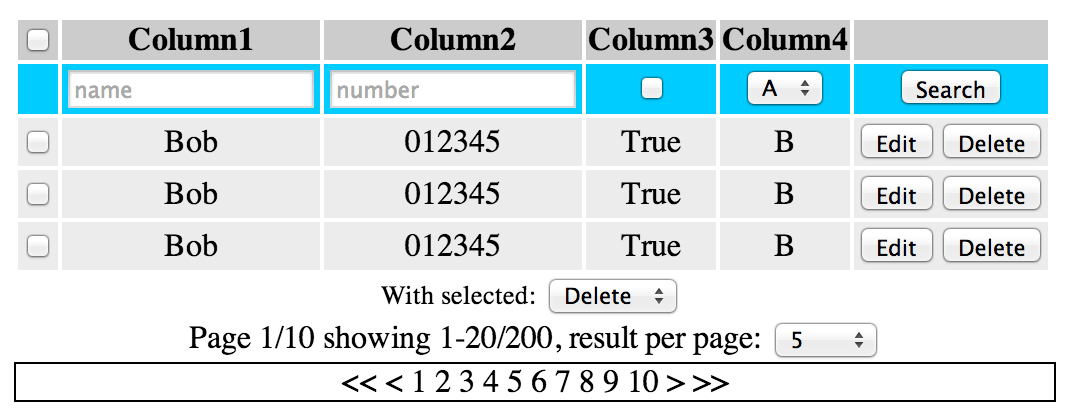
\includegraphics[width=1\textwidth]{img/default_managment_form.png}
		  \caption{Default management table form}
		  \label{default_management_table_form}
		\end{figure}
		The organizer has many similar pages where he has the ability to manage big datasets.
		We will use a similar management table form for all of these pages.
		The first row will also show the names of the fields in the dataset.
		The second row of the column will contain only input fields that will serve as
		search input. For example the organizer can search a user by name and class by
		entering (part) of the pupil's name and the id of the class. The table will
		automatically update when the search button is pressed and will only contain
		rows that satisfy the input query.
		\\
		\\
		The table won't show all rows at al time, but it will use a paging system that
		by default shows only twenty rows at a time.\\
		\\
		Each row also has a select box. When multiple rows are selected, the organizer is
		able to perform multi-actions.
		These multi-actions are useful for when larger groups of pupils require similar
		actions. Clicking a select-box in the column-name row of the table will select
		all the rows on the current page.\\
		\\
		The last column can contain actions like Edit and Delete and those will be
		performed on that row.
	\end{subsection}
\end{section}